% \documentclass{standalone}
% \usepackage{currfile,hyperxmp}

% \input{../tikz_header.tex}

% \begin{document}



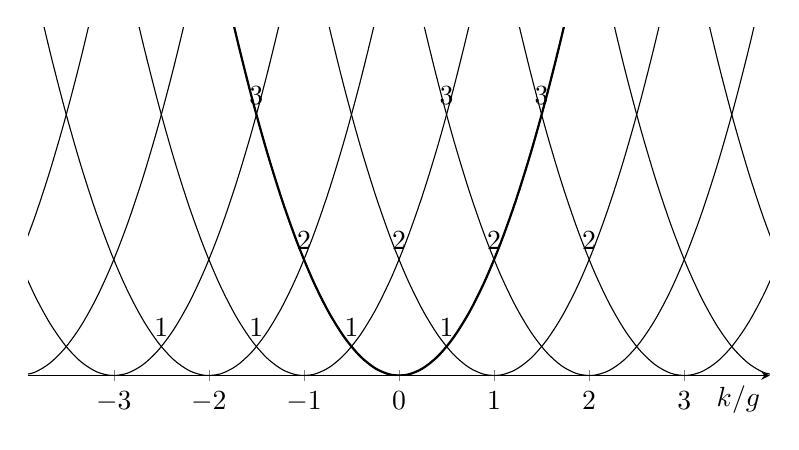
\begin{tikzpicture}
%\useasboundingbox (-1.3,-1.2) rectangle (10.2,4.7);
%\draw (-1,-1) rectangle (4,4);


\begin{axis}[
         width=110mm, height=60mm,
         ymin = 0,
         ymax = 3,
         xmin = -3.9,
         xmax = 3.9,
         axis x line=bottom,
         axis y line=none,
         %xtick = {-2,-1, -0.5, 0, 0.5, 1,2}, xticklabels = {$-2 g$, $-g$, $-g/2$, $0$, $g/2$, $g$, $2g$ },
         %xtick = {-2, -1.5 , -1, -0.5, 0.5, 1,  1.5, 2},
         %xticklabels = \empty,
         %xmajorgrids,
         xlabel = {$k/g$},
         x label style={at={(axis description cs:1,0)},anchor=north east},
         ]

    \pgfplotsinvokeforeach{-11,...,11}{
        \addplot[no marks, color=black, domain = -4:4,samples=50,smooth] {(x- #1)^2};
        }
    
    \addplot[thick, no marks, color=black, domain = -4:4,samples=50,smooth] {(x)^2};

    \node[above] at (-0.5, 0.25) {  1};
    \node[above] at (+0.5, 0.25) {  1};
    \node[above] at (-1, 1) {  2};
    \node[above] at (-1.5, {1.5^2}) {  3};
    \node[above] at (+1.5, {1.5^2}) {  3};
    \node[above] at (+0.5, {1.5^2}) {  3};
  
    \node[above] at (-1.5, 0.25) {  1};
    \node[above] at (-2.5, 0.25) {  1};

    \node[above] at (0,1) {  2};
    \node[above] at (1,1) {  2};
    \node[above] at (2,1) {  2};

    \end{axis}

\end{tikzpicture}

%\end{document}